\documentclass{beamer}
\usetheme{metropolis}           % Use metropolis theme

\usepackage{tikz-cd} % diagramas
\usepackage{leftindex} % diagramas
\usepackage{epigraph} % citacao
\usepackage[portuguese]{babel}
% \usepackage{natbib}
% \usepackage[style=alphabetic, backend=biber, labelalpha]{biblatex}
% \bibliography{References/references}

\usetikzlibrary{positioning}

\newcommand{\bb}[1]{\mathbb{#1}}
\newcommand{\Z}{\bb{Z}}
\newcommand{\Q}{\bb{Q}}
\newcommand{\R}{\bb{R}}
\newcommand{\U}{\bb{U}}
% \newcommand{\C}{\bb{C}}
\newcommand{\ZpZ}{\bb{Z}/p\bb{Z}}
\newcommand{\fit}{Fit}
\newcommand{\ol}[1]{\overline{#1}}
\newcommand{\li}{\leftindex}

\DeclareMathOperator{\fib}{fib}
\DeclareMathOperator{\MAX}{MAX}


\title{{\Large Programação Competitiva}\\ Semana 5: Estruturas de dados}
\date{17 de Setembro, 2025}
\author{Alberto Tavares Duarte Neto}
\institute{Universidade de Brasília}

\usepackage[natbib=true,style=authoryear,backend=bibtex,useprefix=true]{biblatex}
\addbibresource{references.bib}

\beamertemplatenavigationsymbolsempty

\usepackage{multicol}
% \usepackage{amsmath}
% \usepackage[all]{xy}
\usepackage{tikz}
\usepackage[]{minted}

\usepackage{amsfonts, amsthm, amsmath, amssymb}
% \usepackage[bottom=2cm,top=3cm,left=3cm,right=2cm]{geometry}
%\usepackage{empheq}

\numberwithin{equation}{subsection}
\usepackage{hyperref}


\begin{document}
    \maketitle
    \small


    %%% falar de stack e queue
    %%% falar de pq

    %%% sets:

    % falar que eh uma arvore binaria de busca (log n)
    % problema da mediana
    % venice set

    %%% maps:

    % falar que eh um set de pairs

    
    \begin{frame}{Estruturas de dados}
    \metroset{block=fill}

    \begin{block}{Definição}
        Uma {\bf estrutura de dados} é uma maneira de armazenar e organizar dados para facilitar acesso e modificação.
    \end{block}

    Exemplos de estruturas de dados:

    \begin{itemize}
        \item Vetor.
        \item Pilha.
        \item Fila.
        \item Fila de prioridade.
        \item Mapa.
        \item Árvore binária de busca (\textit{set}).
    \end{itemize}

    Não existe uma estrutura ótima para todas as situações. Cada estrutura tem restrições e complexidades diferentes.

\end{frame}


    \begin{frame}{Pilha}
    \metroset{block=fill}

    \begin{block}{Definição}
        Uma {\bf pilha} é uma estrutura onde a remoção remove o elemento mais recentemente inserido.
    \end{block}

    \begin{itemize}
        \item Acesso: $O(1)$.
        \item Inserção: $O(1)$.
        \item Remoção: $O(1)$.
    \end{itemize}

    \begin{block}{Pilha}
        \footnotesize
        \inputminted{cpp}{codigos/pilha.cpp}    
    \end{block}

\end{frame}


    \input{1.2-fila.tex}
    \begin{frame}{Fila de prioridade}
    \metroset{block=fill}

    \begin{block}{Definição}
        Uma {\bf fila de prioridade} é uma estrutura onde a remoção remove o elemento com maior valor.
    \end{block}

    A implementação da fila de prioridade é feita a partir de uma heap de máximo (cf. Cormen, Cap. 6). Por exemplo, uma heap de máximo armazenando os elementos $\{1, 2, 3, 4, 7, 8, 9, 10, 14, 16\}$ é

    \begin{figure}
        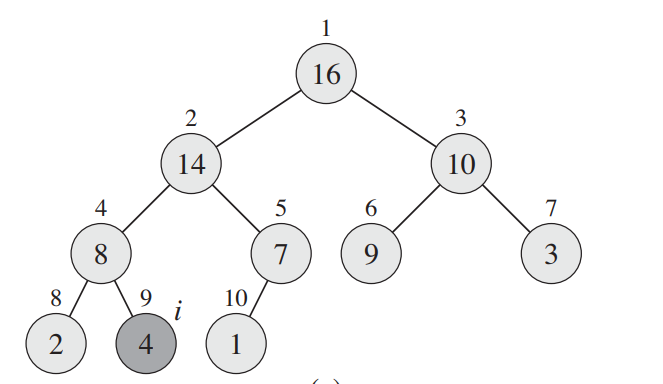
\includegraphics[scale=0.25]{max-heap.png}
    \end{figure}
    
\end{frame}


    \begin{frame}{Fila de prioridade}
    \metroset{block=fill}

    A cada inserção ou remoção, é feito um rebalanceamento na árvore para que sua altura seja sempre $\log n$, onde $n$ é a quantidade de elementos na estrutura. Assim, é possível realizar as operações com as seguintes complexidades:

    \begin{itemize}
        \item Acesso: $O(1)$.
        \item Inserção: $O(\log n)$.
        \item Remoção: $O(\log n)$.
    \end{itemize}

    \begin{block}{Fila de prioridade}
        \footnotesize
        \inputminted{cpp}{codigos/fila-prioridade.cpp}    
    \end{block}
    
\end{frame}



    \begin{frame}{Árvore binária de busca}
    \metroset{block=fill}

    \begin{block}{Definição}
        Seja $T$ uma árvore binária em que cada nó possui um valor. Dizemos que $T$ satisfaz a propriedade de {\bf árvore binária de busca} se, para todo nó $x$ de $T$, vale:
            \begin{itemize}
                \item Se $y$ é um nó na subárvore da esquerda de $x$, então $y.valor \leq x.valor$.
                \item Se $y$ é um nó na subárvore da direita de $x$, então $y.valor \geq x.valor$.
            \end{itemize}
    \end{block}

    O objetivo é manter a árvore com altura balanceada: se a árvore tem $n$ nós, queremos que sua altura seja $\log n$. Assim, a complexidade das operações é

    \begin{itemize}
        \item Acesso: $O(\log n)$.
        \item Inserção: $O(\log n)$.
        \item Remoção: $O(\log n)$.
    \end{itemize}


\end{frame}


    \begin{frame}{Árvore binária de busca}
    \metroset{block=fill}

    Existem algumas técnicas para, após uma inserção ou remoção, rebalancear a árvore com complexidade $O(\log n)$. Veja o capítulo $13$ do Cormen.

    Para uma mesma lista $l$, é possível criar várias árvores binárias de busca possuindo nós com os valores de $l$. Por exemplo, se $l = \{1, 2, 3, 4\}$, então temos

    \begin{columns}
        \begin{column}{0.25\textwidth}
            \begin{tikzpicture}[every node/.style={circle, draw=black}]
                \node {2}
                    child { node {1} }
                    child { node {4} 
                        child {node {3}}
                    }
                ;
            \end{tikzpicture}
        \end{column}
        \begin{column}{0.25\textwidth}
            \begin{tikzpicture}[every node/.style={circle, draw=black}]
                \node {1}
                    child { node {3} 
                        child {node {2}}
                        child {node {4}}
                    }
                ;
            \end{tikzpicture}
        \end{column}
    \end{columns}


\end{frame}
    \begin{frame}{Sets}
    \metroset{block=fill}

    Um \textit{set} em C++ é implementado como uma árvore binária de busca. Temos os seguintes métodos para acessar elementos de um set:

    \begin{itemize}
        \item find(x): retorna um iterator para o elemento $x$, se houver, ou set.end() caso contrário.
        \item lower\_bound(x): retorna um iterator para o menor elemento maior ou igual a $x$, ou set.end() caso contrário.    
        \item upper\_bound(x): retorna um iterator para o menor elemento maior que $x$, ou set.end() caso contrário.
    \end{itemize}

    Para acessar o elemento de um iterator \textit{it}, usamos o operador *: *it.

\end{frame}
    \begin{frame}{Sets}
    \metroset{block=fill}

    \begin{block}{Set}
        \footnotesize
        \inputminted{cpp}{codigos/set.cpp}    
    \end{block}

\end{frame}



\end{document}